% !TEX encoding = UTF-8
% !TEX TS-program = pdflatex
% !TEX root = ../tesi.tex

%**************************************************************
\chapter{Introduzione}
\label{cap:introduzione}
%**************************************************************
\section{La realtà Siav S.p.a.}
\label{sec:realtaSiav}
Siav S.p.a è un'azienda informatica. Propone prodotti che si distinguono specialmente nel campo della gestione e elaborazione documentale digitalizzata. Nata in provincia di Padova nel 1989, negli anni ha subito un'espansione sia strutturale che territoriale: dispone infatti di diverse sedi dislocate in Italia con vari ruoli organizzativi e strategici.

Il target di mercato di Siav è difficile da definire: viste le recenti svolte verso l'ambito della digitalizzazione, sia per obblighi legislativi rispetto alla fatturazione digitale, sia per l'esigenza di comfort nella gestione documentale, la suite di prodotti offerti da Siav vede riscontro di interesse da parte di aziende di tutte le entità.

Nella strutturazione Siav trova un punto di forza, dividendo le competenze per reparto ma aprendo a connessioni per valorizzare le persone: non è infatti infrequente che avvengano collaborazioni o consulenze fra reparti proprio per questa ragione. Sono infatti presenti, oltre ai reparti gestionali e consulenziali, diversi reparti di prodotto, divisi a loro volta in base alla specializzazione rispetto alle partizioni dello stesso.

Nelle giornate di lavoro in presenza e durante alcune riunioni ho avuto modo di conoscere, oltre che i miei colleghi di reparto, qualche membro della sede di Rubano e non. La sensazione che più ho distinto è quella di aver collaborato con persone disposte al dialogo e al confronto indipendentemente dal ruolo che ricoprono. Tale sensazione si è trasformata in certezza una volta cominciato il lavoro in reparto.


%**************************************************************
\section{Il reparto Ricerca e Sviluppo}
\subsection{Di cosa si occupa}
\label{subsec:occupazioneRnd}
Durante l'attività di stage, sono stato inserito nel reparto \acrshort{rnd}\glsfirstoccur che è organizzato come \textit{team} di quattro persone. Esso si occupa di effettuare ricerca sulle tecnologie del domani di Siav. Tramite la collaborazione con i clienti e con le altre sezioni della \textit{software house}, costruiscono prototipi di nuovi prodotti e funzionalità di cui l'azienda vuole studiare utilità e fattibilità.

Ogni componente ha competenze e \textit{background} differenziati. In questo modo il \textit{team} possiede dei riferimenti specializzati su molti fronti, pur spaziando su molteplici settori tecnologici: dal tracciamento e rilevazione in ambito \textit{Process Mining}, alla predizione tramite \acrlong{ml}\glsfirstoccur passando per la ottimizzazione di infrastrutture software e \textit{cloud} per le piattaforme già esistenti.

Come ho introdotto in \S \ref{sec:realtaSiav}, uno dei \textit{core business} di Siav è la produzione di software in ambito dematerializzazione. L'abbandono della documentazione cartacea favorisce una gestione più snella e organizzata di tutto il materiale che usualmente le aziende impiegano e archiviano fisicamente. Una delle conseguenze più dirette di questa trasformazione è la digitalizzazione dei processi che coinvolgevano tali informazioni. Siav offre già delle soluzioni software complete per la produzione e gestione del nuovo materiale digitale. Parallelamente, tramite la sezione \acrshort{rnd}, effettua studi di fattibilità su funzionalità \textit{Process Mining} da integrare nel software in produzione per monitorare questi processi. Per sfruttare al massimo le risorse impiegate, gli studi vengono effettuati dal reparto in modalità \textit{context-free}, studiando le esigenze di potenziali clienti e non limitandosi ai processi documentali.
\begin{figure}[H] 
    \centering 
    
\includegraphics[width=0.45\columnwidth]{immagini/text-mining.png} 
    \caption{Elaborazione documentale - \href{https://pixabay.com/it/users/mcmurryjulie-2375405/?utm_source=link-attribution&amp;utm_medium=referral&amp;utm_campaign=image&amp;utm_content=1476780}{Fonte: PixaBay - mcmurryjulie}}
    \label{fig:elaborazioneDocumentale}
\end{figure}
\newpage
%**************************************************************
\subsection{Il \textit{way of working} del reparto}
\subsubsection{Metodo di sviluppo}
In \acrshort{rnd} vengono attuati alcuni processi con disciplina sfruttando diversi strumenti.
Per verificare frequentemente che la direzione intrapresa dal \textit{team} sia quella corretta ed adattarsi dinamicamente a nuove sfide poste dai clienti o dalla direzione, ogni ciclo di sviluppo segue una metodologia \textit{Agile} ispirata al \textit{framework} \gls{scrum}\glsfirstoccur. Tramite degli incontri settimanali il \textit{team} definisce gli obiettivi da raggiungere che monitora giornalmente con apposite verifiche fra il responsabile e i soggetti interessati.

\begin{figure}[H] 
    \centering 
    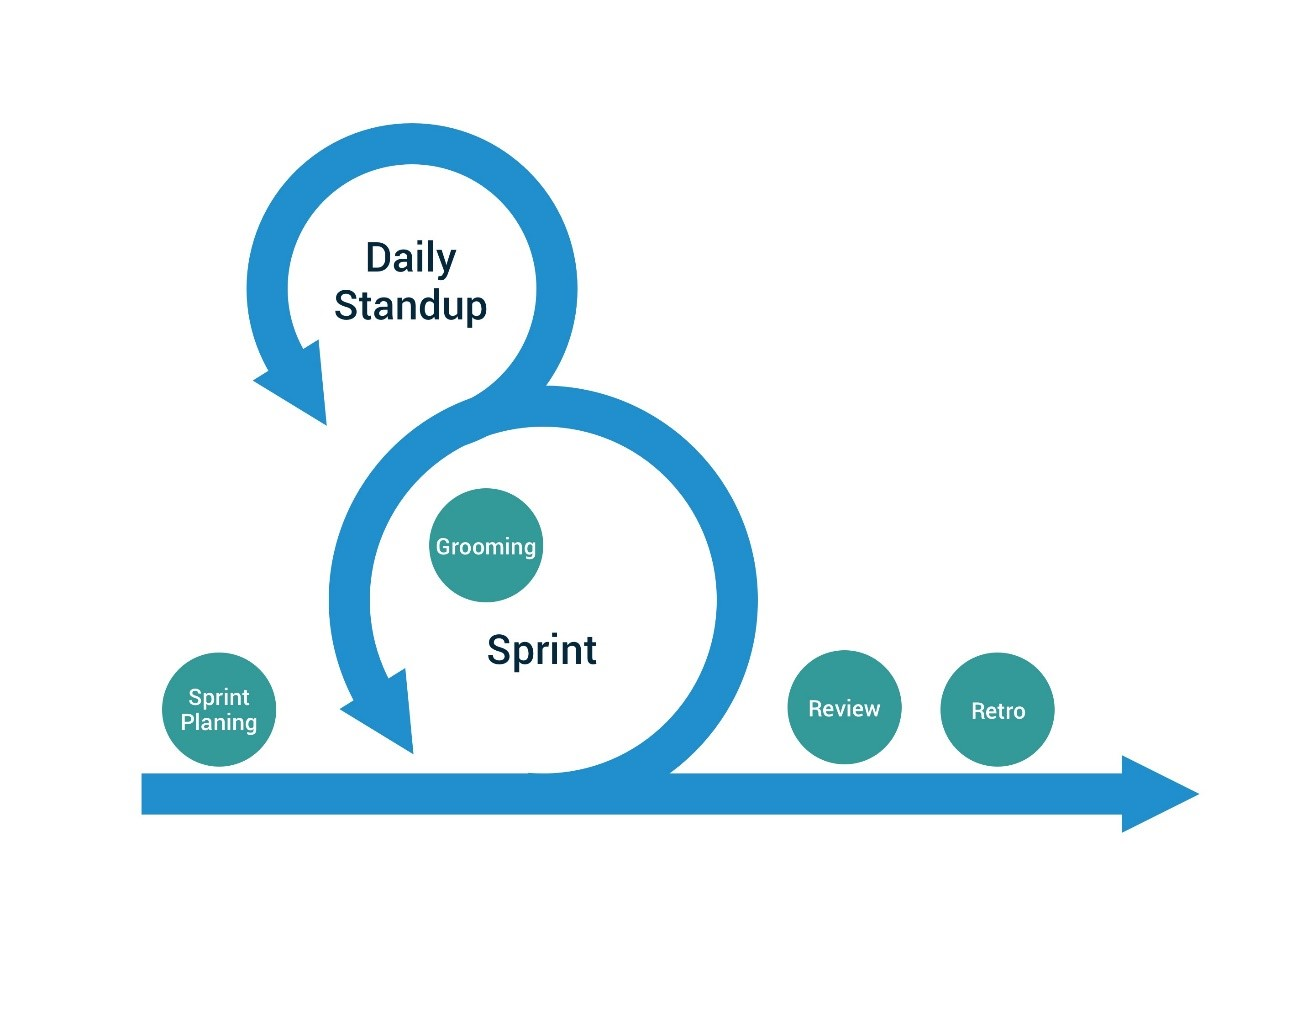
\includegraphics[width=0.9\columnwidth]{immagini/scrum-blog.jpg} 
    \caption{Lo sprint \gls{scrum} - \href{https://www.logicsolutions.com/what-is-scrum-how-it-works/}{Fonte: Logic Solutions}}
    \label{fig:sprintScrum}
\end{figure}

\subsubsection{Strumenti impiegati}
\label{ssec:usedTools}
Per portare a completamento i cicli di sviluppo, il reparto sfrutta diversi strumenti organizzativi e di supporto.
\paragraph{Trello}
Per la gestione di progetto, utilizzano \gls{trello}\glsfirstoccur in versione \textit{enterprise}. Grazie ad esso, è estremamente facile e veloce pianificare e registrare l'impiego di risorse per un progetto, utilizzando un'interfaccia grafica intuitiva e immediata e tramite un tool di reportistica completo.

\paragraph{Evernote}Per la condivisione documentale e per la scrittura collaborativa, usano \gls{evernote}\glsfirstoccur. Tramite esso è possibile creare dei taccuini (anche condivisi) dove raccogliere note di diverso genere ed entità: permette, partendo da una semplice nota di testo, di aggiungere immagini, audio, documenti pdf e \textit{checklists} ad ogni nota.


\paragraph{GitLab}Siav versiona il codice sorgente in \gls{gitlab}\glsfirstoccur \textit{enterprise} ospitato nei server aziendali e raggiungibile da rete interna o tramite connessione alla \acrshort{vpn}\glsfirstoccur aziendale. Nei vari \textit{repository} gli sviluppatori Siav condividono e versionano il codice sorgente in maniera semplice e ordinata.
L'accesso alla rete interna è permesso solamente ai terminali forniti dall'azienda stessa ai suoi dipendenti.

\paragraph{VS Code} Per convenzione, il reparto impiega Microsoft Visual Studio Code come \acrshort{ide}. \'E un ambiente di sviluppo \textit{light-weight} facilmente estensibile con vari \textit{plug-in} dalle svariate funzioni: da vocabolari personalizzati per la \textit{code completion} a software che generano automaticamente \textit{file} di configurazione.

\paragraph{IntelliJ Idea} In alcuni casi, l'editor prodotto da JetBrains viene preferito dal reparto a VS Code perché facilita la configurazione delle attività di \textit{build} e \textit{deployment} e per le funzionalità di controllo delle annotazioni che esso offre. Uno di questi casi è lo sviluppo di applicativo in linguaggio Java.


%**************************************************************
\subsection{Formazione continua}
Per poter affrontare al meglio tutte le richieste effettuate al reparto, responsabile e manager programmano sessioni formative regolarmente. In questo modo permettono l'estensione del bagaglio di competenze basilari di ogni membro, permettendogli così di partecipare ai confronti sulla scelta o sulla modalità di impiego di una tecnologia o di uno strumento. Tali confronti diventano così multidirezionali, non basati sul \textit{knowledgement} del singolo e perciò sicuramente più puntuali.

Nel periodo durante il quale ho svolto lo stage, per esempio, il \textit{team} ha affrontato diverse formazioni su \gls{sagemaker}\glsfirstoccur, un tool di \acrlong{ml} offerto da \acrlong{aws}\glsfirstoccur, parallelamente alle altre attività che coinvolgevano il reparto. Nell'esempio specifico, la formazione è stata effettuata per valutare la fattibilità dell'inserimento di una nuova funzionalità in un software in produzione. Nonostante un componente del \textit{team} sia già in grado di padroneggiare tale servizio, il responsabile ha preferito fornire a tutti la formazione adeguata per discutere in seguito sulla progettazione della struttura che andrà a supportare la nuova funzionalità.

\begin{figure}[H] 
    \centering 
    
\includegraphics[width=0.5\columnwidth]{immagini/team_working.png} 
    \caption{Teamworking - \href{https://pixabay.com/it/users/GraphicMama-team-2641041/?utm_source=link-attribution&amp;utm_medium=referral&amp;utm_campaign=image&amp;utm_content=1453895}{Fonte: PixaBay - GraphicMama-team}}
    \label{fig:teamworking}
\end{figure}
%**************************************************************
\section{Produzione tramite sperimentazione}
\subsection{Perché sperimentare tramite l'attività di stage}
\label{ssec:sperimentareStage}
Una delle filosofie su cui si basa il reparto ricerca e sviluppo, è quella della sperimentazione; negli anni, ha sempre collaborato con gli atenei per effettuare attività di stage in azienda. L'approccio di uno stagista che si avvicina per la prima volta ad un problema aziendale, è un prezioso punto di vista su problemi che il reparto magari ha già affrontato. Un suo valore risiede nel fatto che non è inserito nel contesto e perciò riuscirà sempre a cogliere degli aspetti sui quali non erano state fatte valutazioni. Inoltre, lo stagista ha la volontà, per natura dell'obiettivo che sta perseguendo, di conoscere e imparare, ovviamente, scegliendo delle strade per risolvere i problemi talvolta giuste, talvolta sbagliate.

Durante il lavoro in Siav, tutte le scelte tecniche effettuate dagli stagisti vanno giustificate all'interno del report giornaliero per dare solidità e coerenza alle scelte che affronterà quando il software dovrà andare in produzione. Un esempio di come venga applicata questa filosofia è Bipod.
\subsection{Bipod}
Bipod è il software di \textit{Process Mining} sviluppato da Siav. Ogni funzionalità in esso è stata implementata dal reparto tramite la collaborazione con uno o più studenti. Permette, a partire dai dati aziendali relativi a uno o più processi, di ricostruire dei grafi di processo e di effettuare calcoli sul valore degli indici di processo che l'utente desidera. Questo tramite la formulazione di \acrshort{kpi}\glsfirstoccur. Una volta inserite delle soglie da parte dell'utente, permette di monitorare lo stato di tali indici in formato grafico.
\begin{figure}[H]
    \centering
    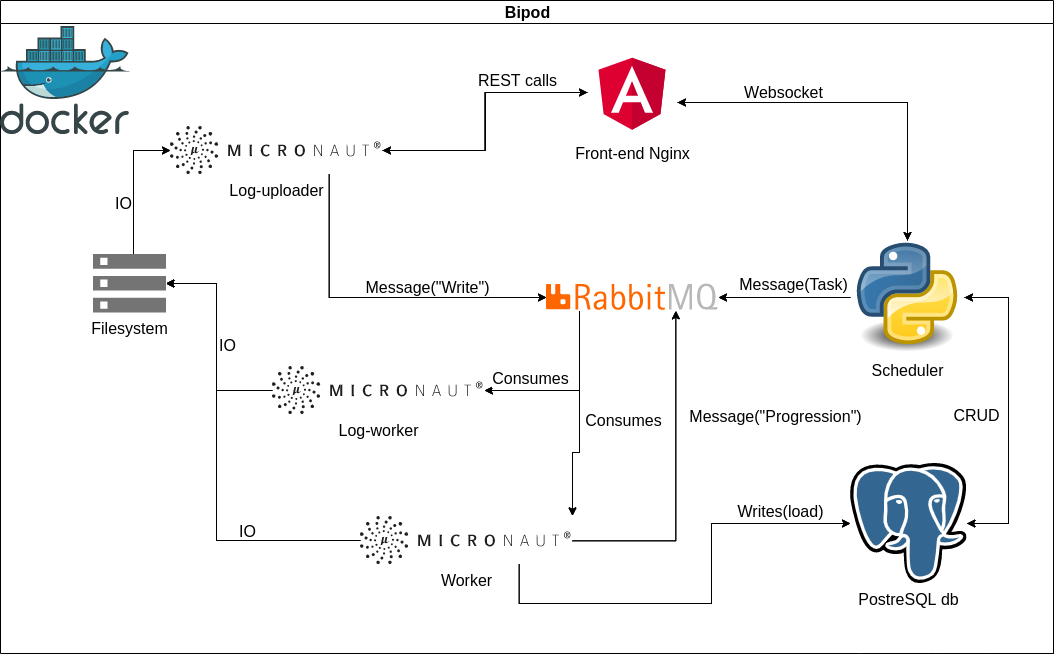
\includegraphics[width=\columnwidth]{immagini/Bipod docker scheme.png}
    \caption{La struttura del sistema Bipod}
    \label{fig:bipodMessages}
\end{figure}

\subsubsection{Tecnologie coinvolte}
\label{ssec:techEnvolved}
\'E un software strutturato costituito da 5 partizioni, ognuna con determinati compiti e funzioni. Coinvolge infatti diverse tecnologie in base alle prerogative di ogni parte:

\paragraph{Docker} Orchestratore di \textit{container}, permette l'esecuzione indipendente di diversi servizi sulla stessa macchina eseguendoli come macchine virtuali indipendenti che comunicano tramite una rete. Grazie alla virtualizzazione è possibile gestire anche diverse istanze dello stesso \textit{container} contemporaneamente

\paragraph{Nginx} \'E un \textit{light-weight} web server che permette la gestione dell'invio di pagine web ai client che le richiedono.

\paragraph{Angular} \textit{Framework} di sviluppo per applicazioni web basato sul linguaggio TypeScript che organizza il codice secondo un paradigma di progettazione che coinvolge \textit{component} e \textit{service}. I primi, come suggerisce il nome, sono dei componenti grafici a loro volta composti da un \textit{template} di vista e un modulo che ne definisce il comportamento; i \textit{service} sono invece dei moduli che offrono un servizio ( per esempio dati, \textit{proxy} remoto o calcolo).In Bipod viene servito da Nginx.

\paragraph{Python} \'E un linguaggio di programmazione estremamente semplice ed intuitivo. Su queste caratteristiche è stata infatti costruita la sua flessibilità. In Bipod è impiegato per lanciare routine periodiche di \textit{monitoring} del carico di sistema e rilevazione dei processi all'interno del \textit{container Scheduler}.

\paragraph{Micronaut} \textit{Framework} di sviluppo per \acrshort{jvm}\glsfirstoccur, permette di sviluppare e testare velocemente microservizi e \textit{serverless applications}. Viene impiegato in Bipod per offrire un servizio di gestione degli indici posti in rilevazione e per registrare uno storico dei valori degli stessi.

\paragraph{PostreSQL} Servizio di \textit{database} relazionale \textit{open source} per l'archiviazione ed interrogazione su grandi moli di dati

\paragraph{RabbitMQ} Servizio di messaggistica che regola la comunicazione tra le parti, necessario per la gestione dei flussi all'interno di un architettura a micro-servizi

%**************************************************************
